\chapter{Discussion}
\label{ch:discussion}


\section{Patterns Observed}
\label{sec:patterns}

\begin{figure}
	\centering
	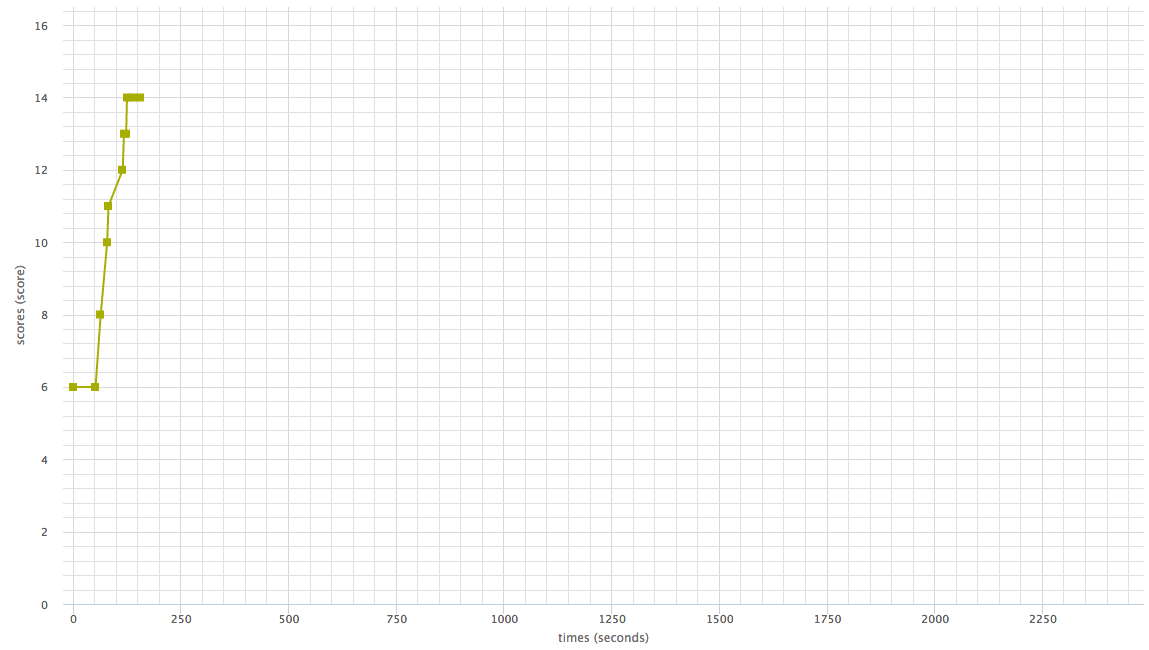
\includegraphics[width=\textwidth]{images/stories/scores-debug-UfaDogfish}
	\caption[Smooth, Rapid Progress of Particle Scores]{Smooth, rapid progress of particle scores, as shown by the student UfaDogfish in the Debugging Activity.}
	\label{fig:smooth_chart}
\end{figure}
Across both activities, three general patterns of particle score progression emerged. The first, called ``smooth'' was a rapid acceleration to the conclusion, where nearly every change improved the score. The ``smooth'' category looks like as if the student already knew the answer, and implemented directly and efficiently. This pattern did allow for slight variation, and smooth-coded projects were not always monotonically increasing, but they were always rapid rises with few changes before the beginning of the upward inflection. An example is shown in Figure \ref{fig:smooth_chart}. Less than a quarter (22\%) of Debugging Activity projects showed this pattern, and just over a quarter (27\%) of the Temperature activity did.

\begin{figure}
	\centering
	\begin{subfigure}{\textwidth}
		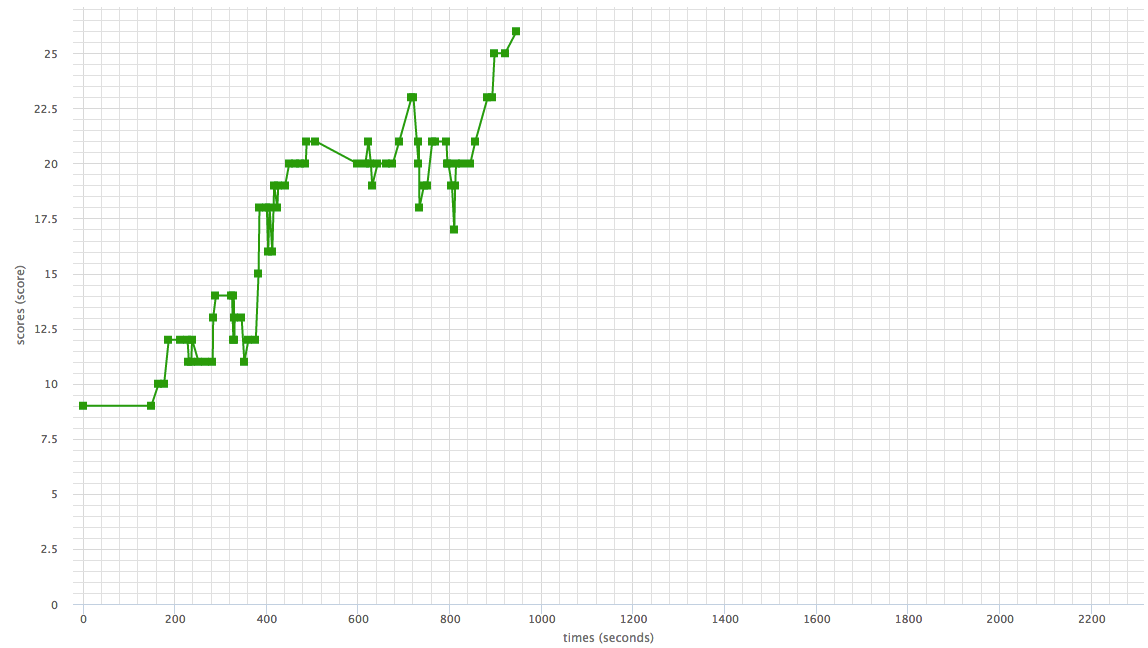
\includegraphics[width=\textwidth]{images/stories/scores-temp-HangzhouTurkey}
		\caption{HangzhouTurkey in the Temperature Activity}
	\end{subfigure}\hfill
	\begin{subfigure}{\textwidth}
		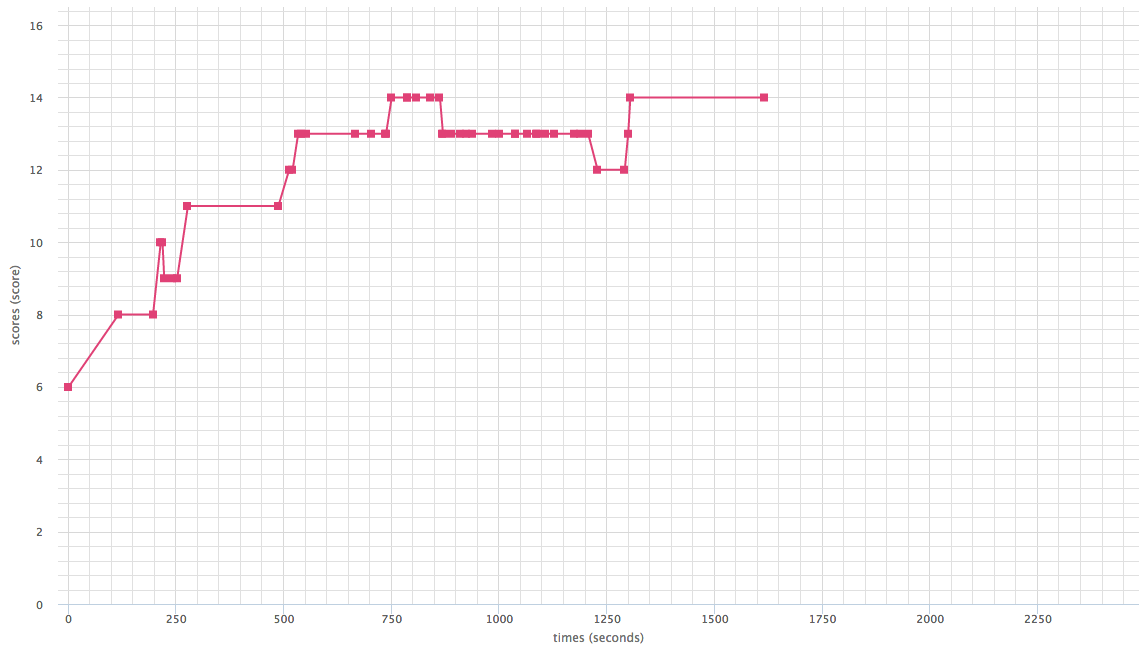
\includegraphics[width=\textwidth]{images/stories/scores-debug-LondonDragonfly}
		\caption{LondonDragonfly in the Debugging Activity}
	\end{subfigure}\hfill
	\caption[``Fits and Starts,'' Typical Progress of Particle Scores]{Two examples of ``Fits and starts,'' demonstrating the typical progress of particle scores.}
	\label{fig:fits_starts_chart}
\end{figure}
The second pattern category was called ``fits and starts'' and represents the most typical trajectory, where the score has periods of progress, non-progress, and sometimes regression, but overall trends upwards and reaches a reasonably successful final state. This was the most broad category, as it was also the one to catch any pattern that was not clearly smooth (above) or flailing (below). Two examples are provided in Figure \ref{fig:fits_starts_chart}, to show the core pattern and some of the allowable variation around it. The Debugging Activity and Temperature Activity projects fell into this category at rates of 49\% and 60\%, respectively. 


\begin{figure}
	\centering
	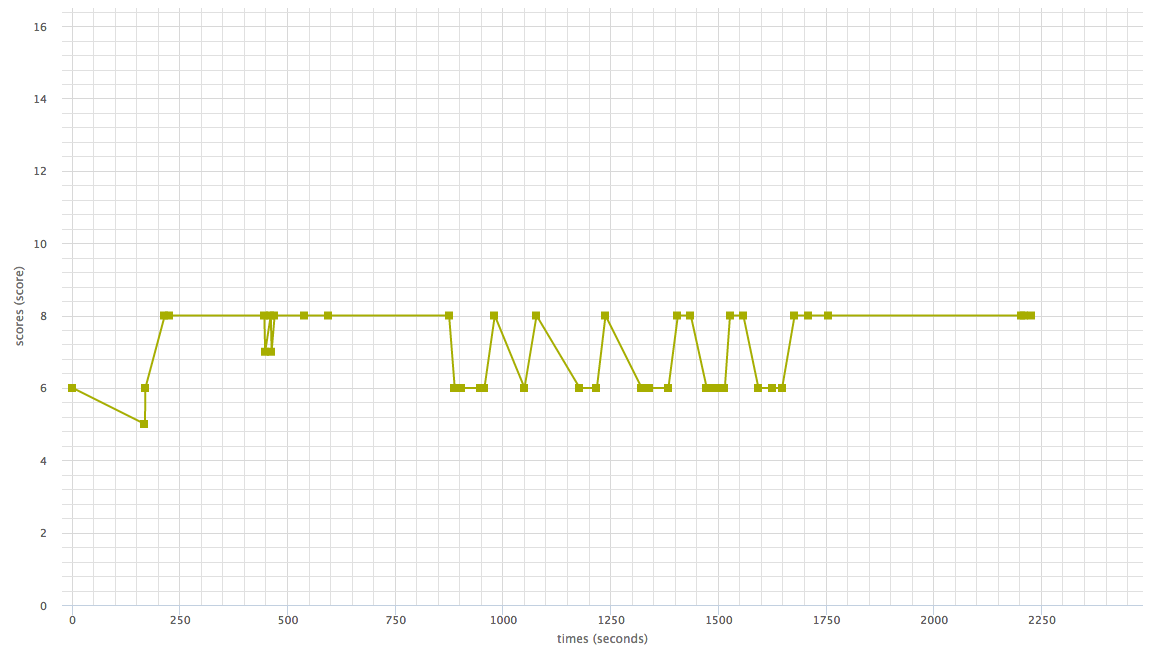
\includegraphics[width=\textwidth]{images/stories/scores-debug-RomePelican}
	\caption[Flailing Pattern, a Lack of Progress of Particle Scores]{Flailing pattern is indicated by a lack of overall progress of particle scores, as shown by the student RomePelican in the Debugging Activity.}
	\label{fig:flailing_chart}
\end{figure}
The third pattern category was ``flailing.'' While the ``fits and starts'' category did allow some flailing behavior, whether score oscillation or non-progress changes, that category always had a generally upwards trend, and resulted in a solution. This category of flailing was reserved for the projects that demonstrated little progress in total, and were entirely flailing behaviors. This pattern is shown in Figure \ref{fig:flailing_chart}. 

A proportion (30\%) of the Debugging Activity projects fell into this category, but, surprisingly, only 13\% of Temperature Activity projects did. We had hypothesized that where the Temperature Activity lacked proper scaffolding there would be more flailing behavior, but the largest category was by far ``fits and starts.'' We can posit that the low rate of apparent flailing at this scale may be due to the aggressive availability of helpers for intervention. The problem may have been sufficiently hard that many students did not even try until they got help from someone. This hypothesis is supported by the wide variation of inflection point, the time where the scores began to increase. Some started right away, while others started nearly at the end of the session period, with many in between. This time translation may be an artifact of the teaching assistants working their way through the classroom, eventually giving everyone the intervention necessary for them to understand and be effective within the problem.

These categories, and the students in each for both activities, is shown in Tables \ref{tab:pattern_names_debug} and \ref{tab:pattern_names_temp}.

\begin{table}
\begin{centering}
	\begin{tabular}{p{\textwidth}}
	\hline \hline
	``Smooth'' (23, 22\%)\\ \hline
		CampoPrairie		
		CiudadWeasel		
		CuiabáGoldfish		
		DetroitShark		
		DortmundBat			
		GorakhpurYak		
		GuayaquilRook		
		HamamatsuFrog		
		JohorGuineaPig		
		KermanshahCockroach1
		LagosRook			
		LibrevilleCrow		
		MendozaAnteater		
		ParisAlligator1		
		PeshawarGnat		
		RangoonBear			
		SantaGrasshopper	
		SeoulOkapi			
		TrujilloLouse		
		TurinFly			
		UfaDogfish			
		VisakhapatnamSheep	
		ZaporizhzhyaFalcon	\\ \hline \hline

	``Fits and Starts'' (51, 49\%)\\ \hline
		AcapulcoDeer		
		CairoCat			
		ChelyabinskSpider	
		ConakryBear		
		CórdobaSalmon	
		DatongPigeon		
		DenverDolphin		
		DhakaClam			
		DhakaEchidna		
		DublinBee			
		FukuokaGoldfinch	
		GuayaquilRook1	
		HangzhouTurkey	
		HangzhouTurkey1	
		HefeiKudu			
		HermosilloSandpiper
		HubliMarten		
		IndoreDogfish		
		IndoreWallaby		
		JinzhouGorilla	
		KaohsiungViper	
		KitakyushuSeal	
		KobeCaterpillar	
		KobeSalamander		
		KuchingCheetah		
		LahoreLapwing		
		LondonDragonfly		
		LusakaOx			
		MoreliaOx			
		MultanFrog			
		MunichTermite		
		NanchangOwl			
		OnitshaWombat
		PermHerring
		PhoenixWeasel
		PointeCheetah
		PueblaVulture
		SeoulSheep
		ShahChinchilla
		SholapurSandpiper
		SurabayaChimpanzee
		TaichungRook
		TaizhouSwallow
		TbilisiKudu
		TijuanaOctopus
		VladivostokCurlew
		WarangalStinkbug
		WroclawRat
		XianAntelope
		YanchengGoose
		ZhangjiakouSardine		\\ \hline \hline
	``Flailing'' (31, 30\%)\\ \hline
		CalgaryHyena
		ChongjuOwl
		HachiojiPeafowl
		HamadanMouse
		HaoraDragonfly
		KadunaAlpaca
		KermanshahCockroach
		KhabarovskBoar
		MakhachkalaWasp
		MultanVulture
		NagpurAlpaca
		NiyalaAlligator
		OkayamaMarten
		OklahomaGiant
		ParisAlligator
		PhiladelphiaWoodpecker
		QuerétaroMule
		QuitoShark
		RomePelican
		SapporoWoodcock
		SarajevoDuck
		SurabayaTermite
		SuwonGoldfish
		TaiyuanDinosaur
		TianjinAlbatross
		TripoliSandpiper
		ValenciaFox
		VijayawadaOtter
		WarsawCrocodile
		XuzhouLoris
		YaroslavlCattle	\\ \hline

	\end{tabular}
	\caption[Categories of Progress Patterns for the Debugging Activity and the Students in them]{Categories of Progress Patterns for the Debugging Activity and the Students in them.}
	\label{tab:pattern_names_debug}
\end{centering}
\end{table}

\begin{table}
\begin{centering}
	\begin{tabular}{p{\textwidth}}
	\hline \hline
	``Smooth'' (8, 27\%)\\ \hline
		DortmundBat
		HubliMarten
		KermanshahCockroach
		MendozaAnteater
		RangoonBear
		TbilisiKudu
		UfaDogfish
		ZaporizhzhyaFalcon
		\\ \hline \hline
	``Fits and Starts'' (18, 60\%)\\ \hline
		DatongPigeon
		FukuokaGoldfinch
		HangzhouTurkey
		KobeSalamander
		LondonDragonfly
		PhoenixWeasel
		PointeCheetah
		PueblaVulture
		QuerétaroMule
		ShiheziBat
		SurabayaChimpanzee
		SurabayaTermite1
		TaiyuanDinosaur
		TaizhouSwallow
		VeracruzDotterel
		VisakhapatnamSheep1
		VladivostokCurlew
		WroclawRat
		\\ \hline \hline
	``Flailing'' (4, 13\%)\\ \hline
		Rostov-na-DonuLapwing
		Rostov-na-DonuLapwing1
		SurabayaTermite
		VaranasiOstrich
		\\ \hline

	\end{tabular}
	\caption[Categories of Progress Patterns for the Temperature Activity and the Students in them]{Categories of Progress Patterns for the Temperature Activity and the Students in them.}
	\label{tab:pattern_names_temp}
\end{centering}
\end{table}



\section{Detailed Case Analysis}
\label{sec:case_analysis}
A selection of student projects were chosen for case analysis, presented here. They were selected to represent the good, the bad, and the interesting. For each, a chart is provided that shows their score in the activity over time. These charts are drawn to the same scale within an activity to allow them to be visually comparable. Additionally, some samples from the code playback history are included, which represent highlights of the student's actual code states to provide concrete explanation for the particle scores.

\subsection{The Good: CampoPrairie}
\begin{figure}
	\centering
	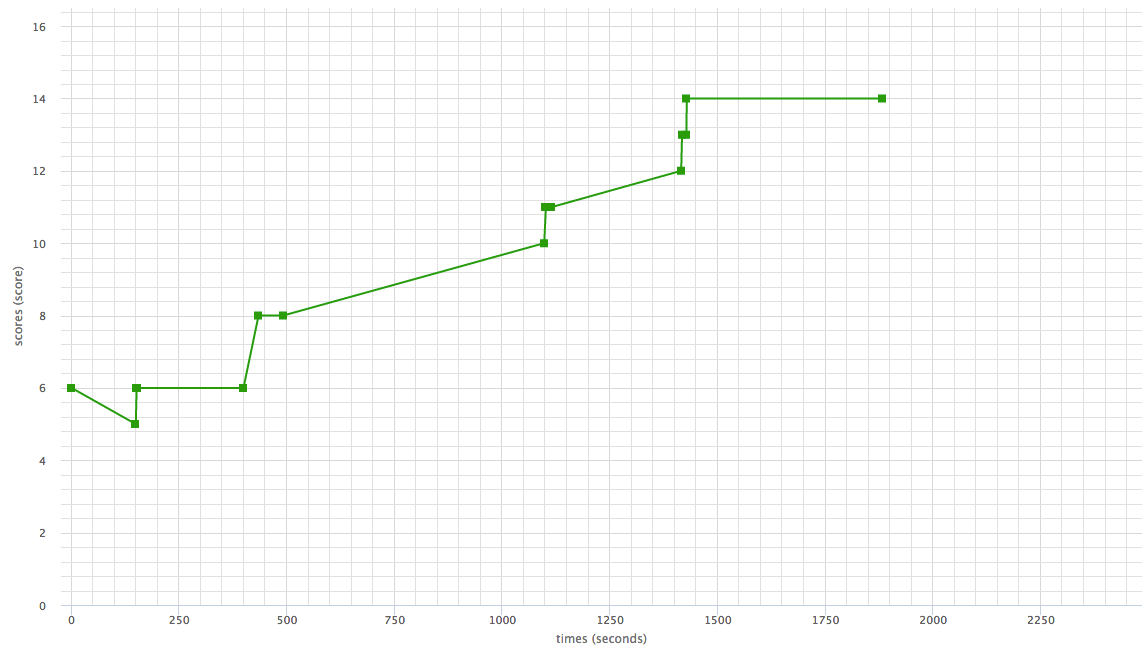
\includegraphics[width=\textwidth]{images/stories/scores-debug-CampoPrairie}
	\caption[Good: CampoPrairie Debugging Activity Particle Scores]{Good: CampoPrairie Debugging Activity Particle Scores.}
	\label{fig:CampoPrairie_chart}
\end{figure}

\begin{figure}
	\centering
	\begin{subfigure}{.45\textwidth}
		\fbox{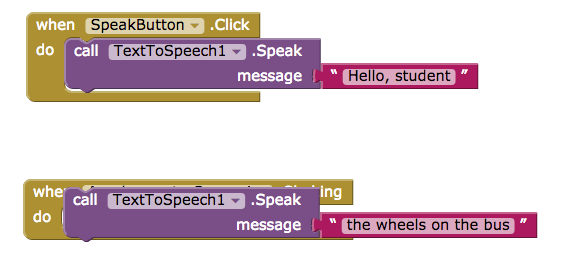
\includegraphics[width=\textwidth]{images/stories/blocks-debug-CampoPrairie/1}}
		\caption{2:29 block accidentally knocked out of place} 
	\end{subfigure}\hfill
	\begin{subfigure}{.4\textwidth}
		\fbox{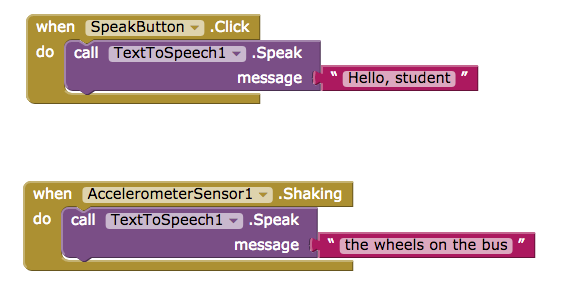
\includegraphics[width=\textwidth]{images/stories/blocks-debug-CampoPrairie/2}}
		\caption{2:31 block knocked back in} 
	\end{subfigure}
	\begin{subfigure}{.45\textwidth}
		\fbox{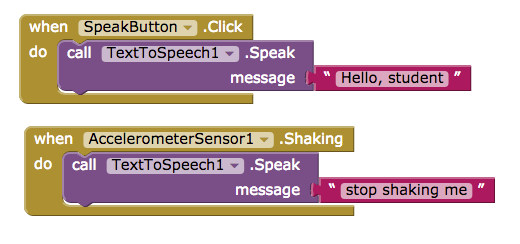
\includegraphics[width=\textwidth]{images/stories/blocks-debug-CampoPrairie/3}}
		\caption{7:14 first bug solved} 
	\end{subfigure}\hfill
	\begin{subfigure}{.45\textwidth}
		\fbox{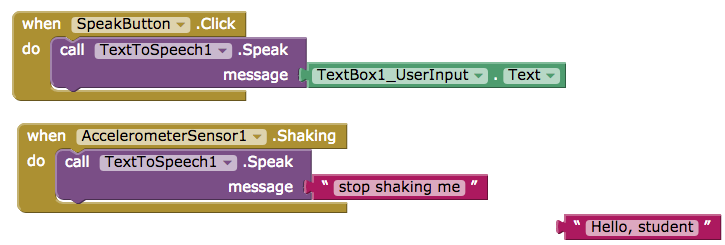
\includegraphics[width=\textwidth]{images/stories/blocks-debug-CampoPrairie/4}}
		\caption{18:21 second bug solved} 
	\end{subfigure}\hfill
	\begin{subfigure}{.45\textwidth}
		\fbox{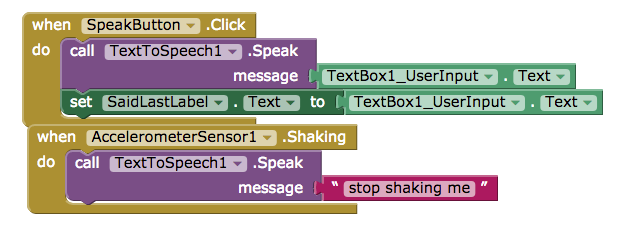
\includegraphics[width=\textwidth]{images/stories/blocks-debug-CampoPrairie/5}}
		\caption{23:48 final bug solved} 
	\end{subfigure}

	\caption[Good: CampoPrairie Debugging Activity Blocks Samples]{Good: CampoPrairie Debugging Activity Blocks Samples. This student completed the activity with minimal difficulty.}
	\label{fig:CampoPrairie_blocks}
\end{figure}

From the Debugging Activity, the assessor looking at blocks playback declared this student ``knew exactly what to do,'' and was coded as ``great'' efficacy. However, this student did not attempt the most difficult subgoal. This student is representative of the typical successful path for this activity. The observation that they quickly ascertained, or already knew, the strategy is supported by the score chart in Figure \ref{fig:CampoPrairie_chart}, which shows a quick and nearly monotonic progression towards the final state. This student reached the solution state in just under 24 minutes.

The brief regression at the beginning of their path is a common and trivial mistake, where a valid block was momentarily knocked out of its parent block, and then quickly re-inserted. This can be seen in the block playback samples in Figure \ref{fig:CampoPrairie_blocks}.


\subsection{The Bad: YaroslavlCattle}
\begin{figure}
	\centering
	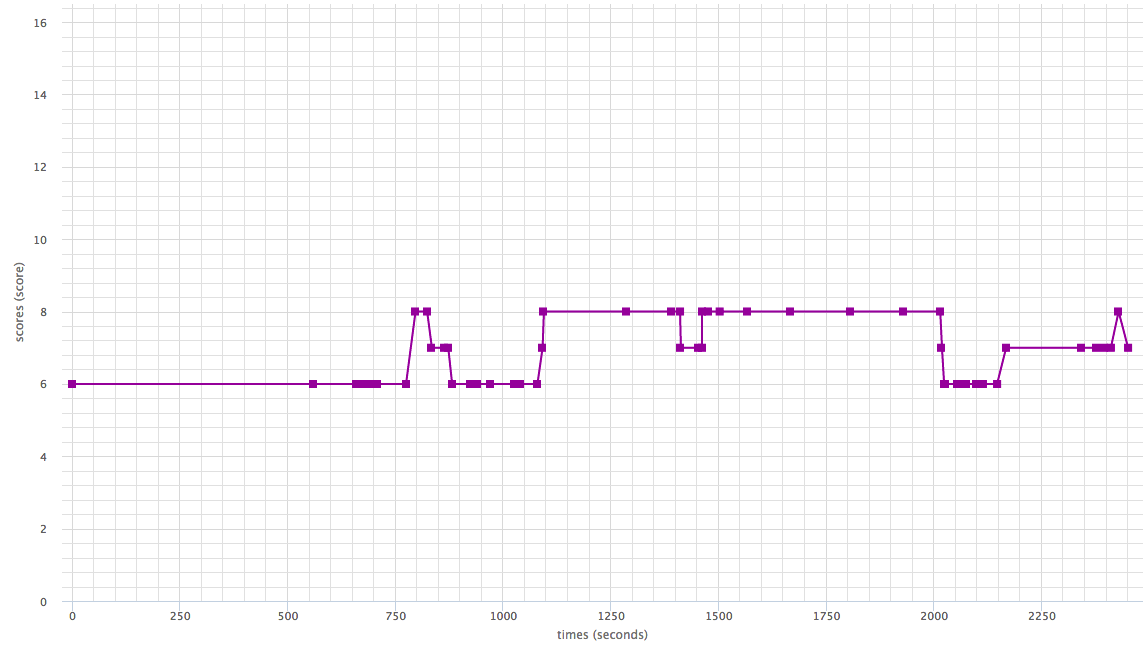
\includegraphics[width=\textwidth]{images/stories/scores-debug-YaroslavlCattle}
	\caption[Bad: YaroslavlCattle Debugging Activity Particle Scores]{Bad: YaroslavlCattle Debugging Activity Particle Scores. This student never progressed more than trivially, despite trying for over 30 minutes.}
	\label{fig:YaroslavlCattle_chart}
\end{figure}

\begin{figure}
	\centering
	\begin{subfigure}{.45\textwidth}
		\fbox{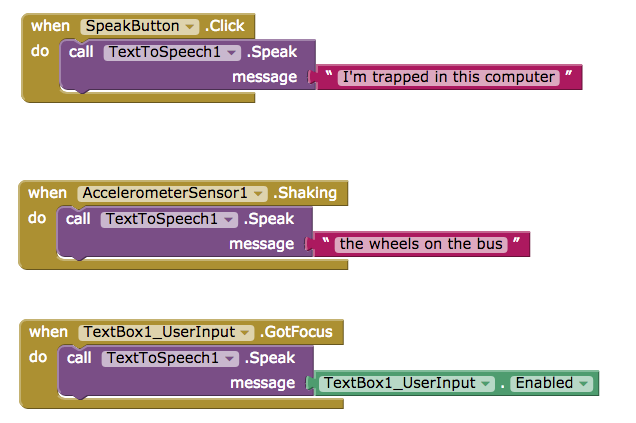
\includegraphics[width=\textwidth]{images/stories/blocks-debug-YaroslavlCattle/1}}
		\caption{11:31 introduced irrelevant \emph{GotFocus} event handler, and populated it with an irrelevant property getter.}
	\end{subfigure}\hfill
	\begin{subfigure}{.4\textwidth}
		\fbox{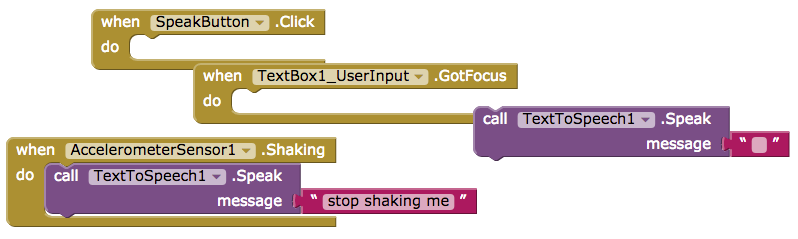
\includegraphics[width=\textwidth]{images/stories/blocks-debug-YaroslavlCattle/2}}
		\caption{14:24 after deleting it, re-introduced the same event handler.} 
	\end{subfigure}
	\begin{subfigure}{.45\textwidth}
		\fbox{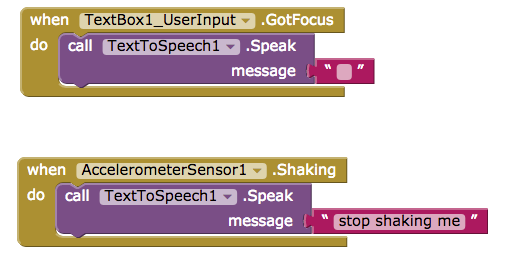
\includegraphics[width=\textwidth]{images/stories/blocks-debug-YaroslavlCattle/3}}
		\caption{16:10 effectively back at the start, a state revisited many times.} 
	\end{subfigure}\hfill
	\begin{subfigure}{.45\textwidth}
		\fbox{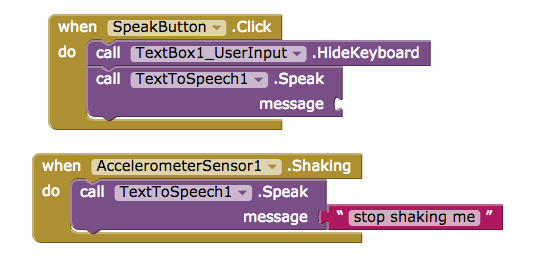
\includegraphics[width=\textwidth]{images/stories/blocks-debug-YaroslavlCattle/4}}
		\caption{23:31 introduced irrelevant \emph{HideKeyboard} block} 
	\end{subfigure}\hfill
	\begin{subfigure}{.45\textwidth}
		\fbox{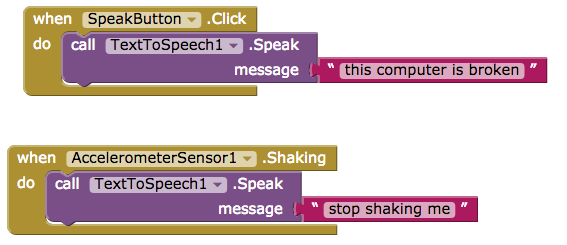
\includegraphics[width=\textwidth]{images/stories/blocks-debug-YaroslavlCattle/5}}
		\caption{26:07 non-topical text entry} 
	\end{subfigure}\hfill
	\begin{subfigure}{.45\textwidth}
		\fbox{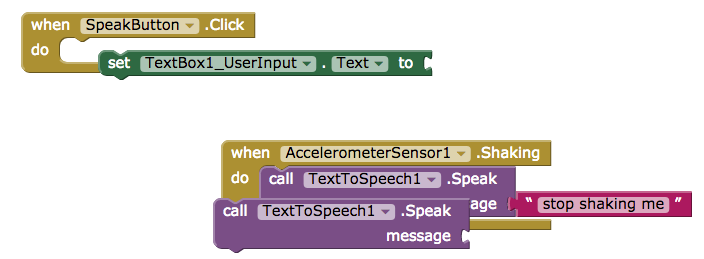
\includegraphics[width=\textwidth]{images/stories/blocks-debug-YaroslavlCattle/6}}
		\caption{40:51 final, inconsistent state} 
	\end{subfigure}

	\caption[Bad: YaroslavlCattle Debugging Activity Blocks Samples]{Bad: YaroslavlCattle Debugging Activity Blocks Samples. This student flailed considerably and made only minor progress.}
	\label{fig:YaroslavlCattle_blocks}
\end{figure}
This student flailed heavily in the Debugging Activity, and appeared to lack traction in understanding the problem. From viewing the blocks playback (Figure \ref{fig:YaroslavlCattle_blocks}), this student repeatedly attempted to construct the same incorrect blocks assembly. They also wrote off-topic prose into text literals, including, at one point, the entirety of the poem ``Twinkle Twinkle Little Star,'' and later, the theme song from the Mickey Mouse Club. This behavior of off-topic text was observed occasionally, and we posit that it is an indicator of lack of traction in the problem. This may be a detectable feature suitable for the teacher's classroom console. An intervention from a teacher or assistant was likely necessary for this student, who never accomplished more than the simplest subgoal. 


\subsection{Interesting: WarangalStinkbug}
\begin{figure}
	\centering
	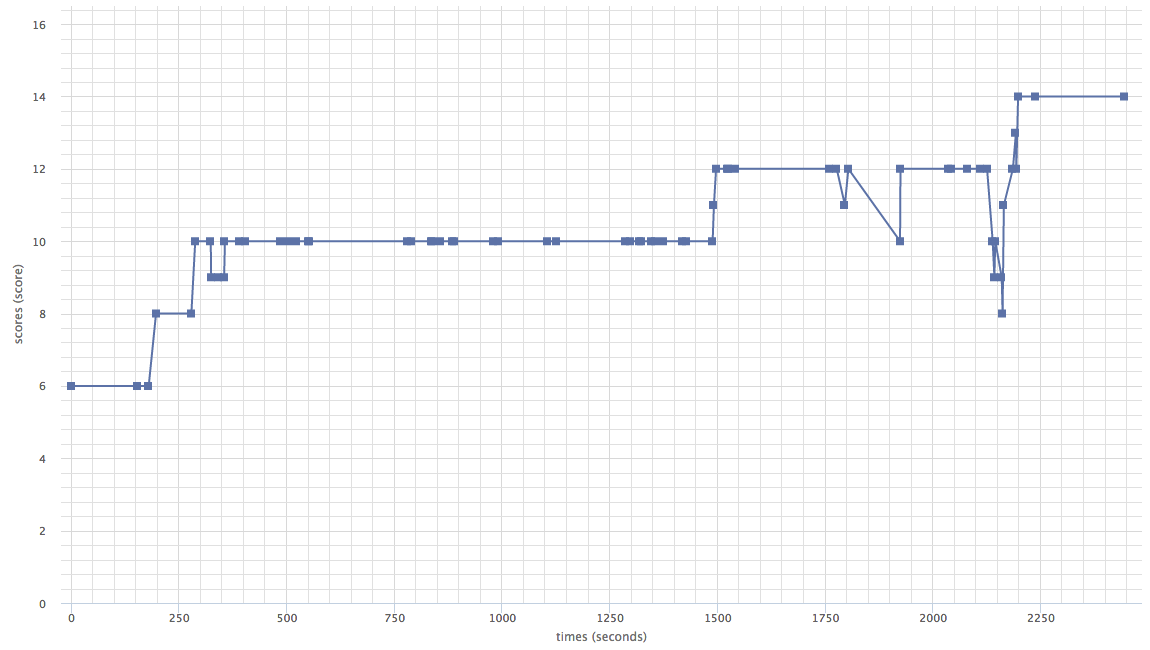
\includegraphics[width=\textwidth]{images/stories/scores-debug-WarangalStinkbug}
	\caption[Bad: YaroslavlCattle Debugging Activity Particle Scores]{Bad: YaroslavlCattle Debugging Activity Particle Scores. This student flailed initially, then was later successful.}
	\label{fig:WarangalStinkbug_chart}
\end{figure}
In the Debugging Activity, a student was observed via playback assessment with ``some flailing in the beginning'' and later success. This was coded as both ``flailing'' and ``good efficacy,'' and that duality makes for a compelling case to analyze. This student started off well at the very beginning, and quickly solved the first bug, and the achieved the simple version of the second bug's solution. After that, this student was unable to make progress for over 20 minutes, during which time they added and deleted a variety of unrelated blocks in turn. This student eventually started making incremental progress. The quick drops in score, followed by immediate return, were caused by a set of blocks that were momentarily removed from their proper context, and then re-inserted. This behavior is common, so large drops in score that are short in duration are not interesting features.


\subsection{Interesting: DenverDolphin \& YanchengGoose}
\begin{figure}
	\centering
	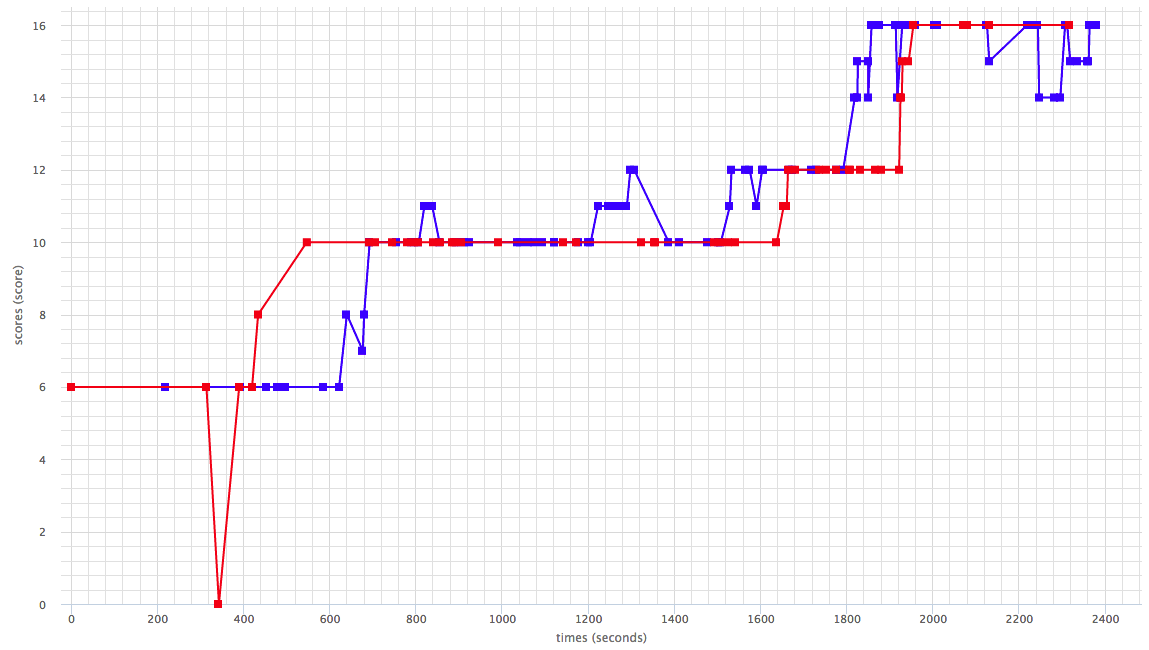
\includegraphics[width=\textwidth]{images/stories/scores-debug-dolphin-goose}
	\caption[DenverDolphin \& YanchengGoose Debugging Activity Particle Scores]{DenverDolphin (blue) \& YanchengGoose (red) Debugging Activity Particle Scores. These were the only students to solve or nearly solve the final subgoal of the activity.}
	\label{fig:dolphin_goose_chart}
\end{figure}
\begin{figure}
	\centering
	\begin{subfigure}{.45\textwidth}
		\fbox{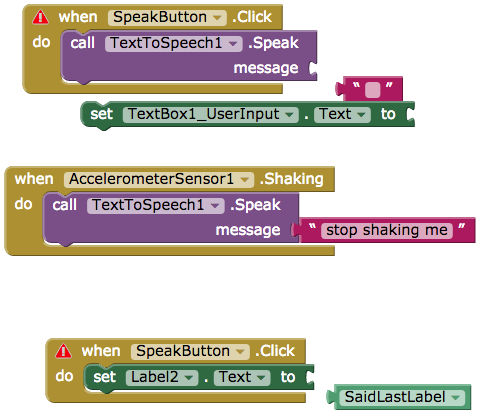
\includegraphics[width=\textwidth]{images/stories/blocks-debug-DenverDolphin/1}}
		\caption{25:04} %frame 130
	\end{subfigure}\hfill
	\begin{subfigure}{.4\textwidth}
		\fbox{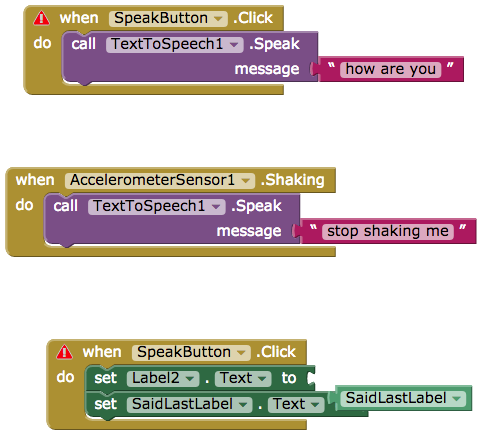
\includegraphics[width=\textwidth]{images/stories/blocks-debug-DenverDolphin/2}}
		\caption{26:08} %frame 142
	\end{subfigure}
	\begin{subfigure}{.45\textwidth}
		\fbox{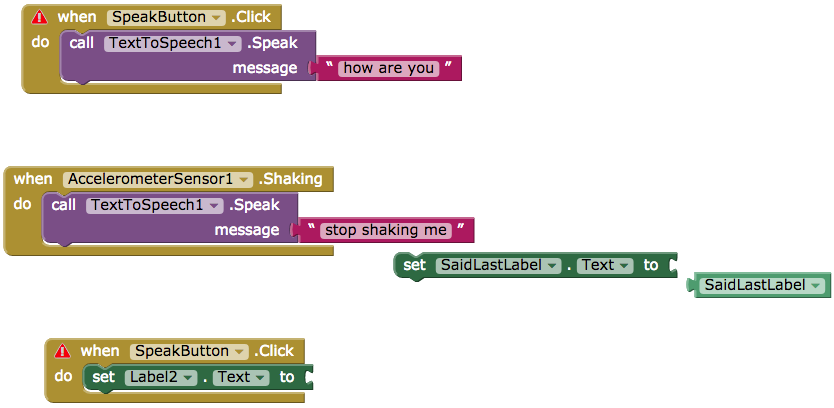
\includegraphics[width=\textwidth]{images/stories/blocks-debug-DenverDolphin/3}}
		\caption{26:43} %frame 159
	\end{subfigure}\hfill
	\begin{subfigure}{.45\textwidth}
		\fbox{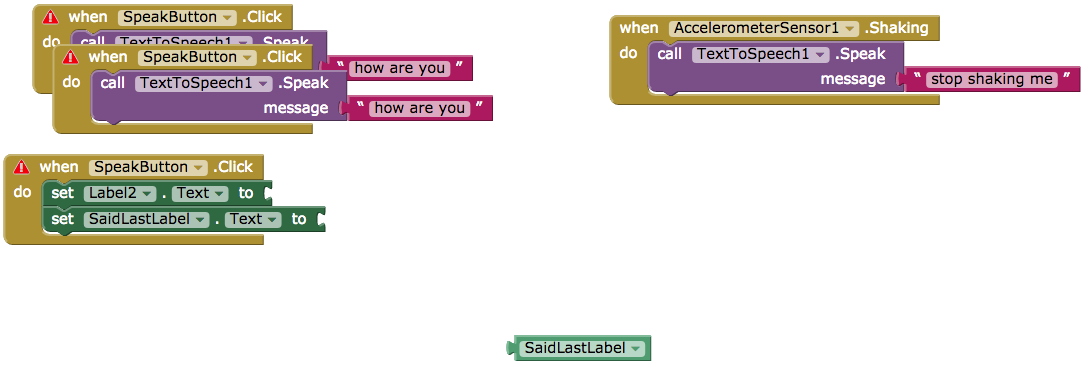
\includegraphics[width=\textwidth]{images/stories/blocks-debug-DenverDolphin/4}}
		\caption{29:36} %frame 181
	\end{subfigure}\hfill
	\begin{subfigure}{.45\textwidth}
		\fbox{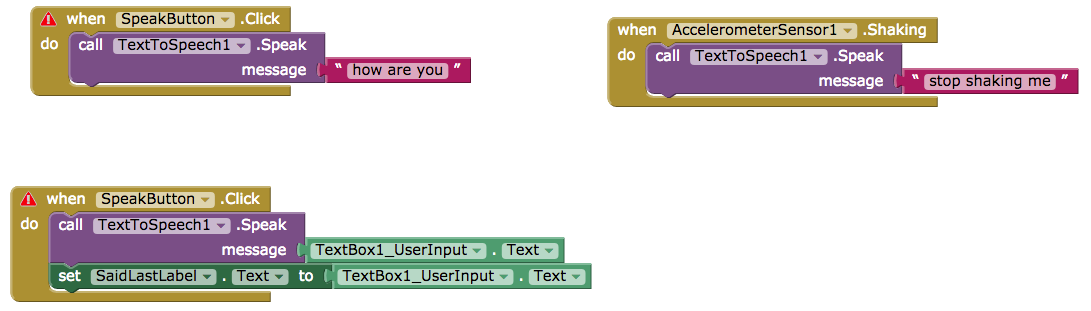
\includegraphics[width=\textwidth]{images/stories/blocks-debug-DenverDolphin/5}}
		\caption{32:21} %frame 217
	\end{subfigure}\hfill
	\begin{subfigure}{.45\textwidth}
		\fbox{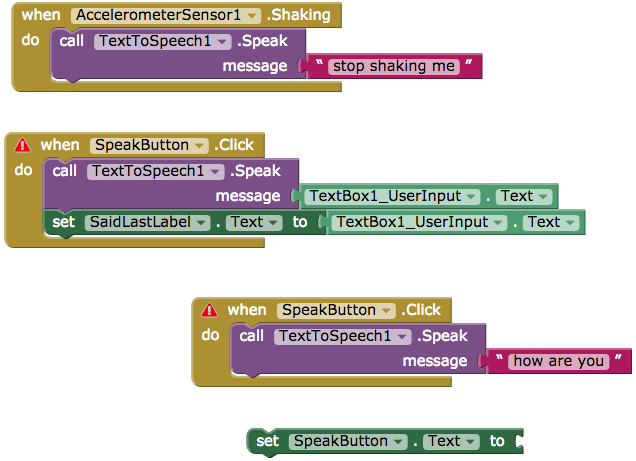
\includegraphics[width=\textwidth]{images/stories/blocks-debug-DenverDolphin/6}}
		\caption{39:46 and final state}
	\end{subfigure}

	\caption[DenverDolphin Debugging Activity Blocks Samples]{DenverDolphin Debugging Activity Blocks Samples, showing the final 15 minutes of work. This student neglected to delete duplicate \emph{SpeakButton.click} handler, but otherwise had the entire activity solved.}
	\label{fig:dolphin_blocks}
\end{figure}

Two students nearly completed the entire Debugging Activity, but had an artificially high particle score, demonstrating a current weakness in the implementation of the particle analysis technique. 

Student DenverDolphin was coded as from blocks playback with ``extreme flailing,'' and judging from Figure \ref{fig:dolphin_goose_chart}, that assessment was correct. This student experienced long periods of activity with no forward progress, and many points of momentary progress followed by regression. YanchengGoose was similar, with a completely flat period of activity from 546 to 1637 seconds, a period of over 18 minutes with no forward progress. Both of these students, however, appeared to slowly worked their way up to the common solution as they approached thirty minutes, and then quickly found their way to an even higher particle score. The students definitely exhibited flailing behavior, but their non-productive behavior did eventually give way to a solution. However, an additional misunderstanding caused both students to access a weakness in the current particle analysis implementation, creating an artificially high score while not solving the final problem.

Upon inspection of the blocks playback, DenverDolphin never actually solved the final bug completely, though came incredibly close. They experimented over a period of about 10 minutes, slowly bringing out more of the relevant blocks, and then constructed the entirely correct event handler and actions. Sadly, they never deleted the old event handler that the new one superseded. App Inventor requires each event handler be unique, and when it encounters duplicates, both are labeled with an error indicator and both are ignored. This student was one small realization away from completing the bug they labored against. A sampling of this student's activity in the final 15 minutes of their session can be seen in Figure \ref{fig:dolphin_blocks}. YanchengGoose exhibited the same behavior, was caught on the same stumbling block, and triggered the same score-inflation weakness. 

As there are three subgoal in the Debugging Activity, there are three separate goal tests, whose scores are summed. If all were executed at the same time, the maximum score would be 16. But that would be impossible with working solutions, as solutions to successive goals actually supersede previous ones, deprecating older code structures. With that, a perfect solution is actually a score of 14. A score of 16 demonstrates a current weakness with the analysis, that a solution can still be over-represented, artificially inflating the score by a small amount.



\section{Evaluating the Classroom Console}
\label{sec:console_evaluation}

% assert console is good, using:
%	Teacher "focus group" feedback
%	Comparison against design goals from literature - Dillenbourg
The researchers recruited a small group of instructors who use App Inventor in their classrooms to see, discuss, and evaluate the Classroom Console. They were interviewed individually, where they were shown the some brief background, the particle assessment concept, a demonstration of the Console. Their reactions were overwhelmingly positive, where the most common question was a form of ``when can I use this?'' The instructors also provided criticism, identified potential weaknesses in the design, and engaged in discussion on how to overcome those weaknesses. One instructor, during the demonstration said, ``I can see right now two students I want to go talk to.'' These discourse are summarized below.

The focus group instructors had two middle school teachers, two middle and high school specialty teachers, two high school and undergraduate instructors, and one undergraduate professor in charge of five lab sections. Their localities included the United States east coast and Midwest, and South America. 

Concerns raised by teachers: 
\begin{itemize}
\item Easily identifies ``needy'' students, who ask for help immediately without first trying on their own. %TODO there is definitely a term for this
\item Similarly, this tool makes it easy to identify high-performing students who can be tasked to help their struggling peers. (Researchers did not realize the tool could be used to identify exemplary performance just as easily as flailing.) 
\item The above matching feature could be automated, in the style of \citet{Diana:2017:IDR:3027385.3027441}.
\item Sometimes you only see students every 8-9 school days, so catching idle periods of mere minutes can be critical. 
\item It is possible for a student who is disengaged to be sitting next to an engaged student, and they both look like they're engaged.
\item When a student returns from a bathroom break, the tool can help assess how quickly they resume engagement.
\item Greatly aids cases where students don't do anything because they know they can get away with it.
\item Training instructors to use the tool may be non-trivial, especially when requiring them to develop their own activities with it. 
\item As the tool is an inexact proxy, experience with the tool may increase the instructor's efficacy with it.
\item High school students are especially afraid to fail, so they often choose not to try anything. This helps identify that behavior.
\item Student feedback often includes the complaint that they did not get enough attention. They could be feeling frustration that the instructor is not seeing, and this helps the instructor gain access into that.
\end{itemize}

Requested Features
\begin{itemize}
\item An automated flag to visually highlight students who are currently exhibiting significant flailing behavior.
\item Flexibility in timeout bar. Some activities and classrooms will have different time frames that would be considered concerning.
\item Treatment for score regression, which is currently not highlighted. 
\item Take the start point with gift code into consideration, and flag the teacher if the student drops below that point, as they have broken their starting configuration and likely need help restoring it.
\item History so teachers can replay or otherwise visual past classroom sessions, and compare them over time. Line chart of the session.
\item Reporting to demonstrate a student's progress in labs over time, suitable for program assessment. 
\item Control over layout, so student locations in Console reflect the seating plan of the classroom.
\item Ability to define your own activities and their corresponding solution particles.
\item Pseudo-anonymized student identifiers, such that the console could be displayed on the projector while the teacher moves around the room.
\end{itemize}

One analysis idea presented by an instructor was to display the \emph{number of attempts} at a certain point of a problem, which would allow the teacher to expect and allow a certain number of attempts before requiring intervention. This method would require further work to better define what an ``attempt'' should mean in general context, and in an activity-specific context.

The instructors were overall excited about the tool, and raised real-world concerns that could further inform the design of the Classroom Console. The instructors declared that the design was ready for prototype use, all citing their desire to use it to enhance their teaching practice.


\section{Conclusions}
\label{sec:conclusions}
A ``flailing detector'' to aid teachers in real-time classroom orchestration is possible when the problem is constrained to known activities with predictable solutions. The particle analysis method delivers a lightweight, good-enough metric to deliver this visual aid in real time. In post-hoc analysis, particle analysis data can be visualized differently to ascertain the trajectories experienced by students. In real time and post-hoc, the visualizations of the particle analysis data lend themselves to easy interpretation of student progress within their activities. Post-hoc tools such as those in this study were requested by teachers while evaluating the real-time console. A package of tools to enable real-time assessment and deeper analysis and reporting after the fact is in demand for teachers who use programming exercises (labs) in the classroom. A number of additional features were identified that would further improve the accuracy of the particle analysis method, such as looking for off-topic strings as a sign of lack of problem traction. Many language- and implementation-specific improvements were also identified to improve the method. This method and its tools are not heavily dependent on language-specific features or work flows, and can be ported to work with any Blockly-based language immediately, and can be used to inform particle analysis implementations in other block, visual, and textual language environments.

%\section{Recommendations} 
% \label{sec:recommendations}
% We do not recommend using git as a database. Further recommendations of legitimate scientific and educational merit will be added as part of the full dissertation.


\section{Future Work}
\label{sec:futurework}

As previously mentioned, there is ample future work to be done in understanding the reasoning behind behavior choices, with particular support to mis-attribution of failure and success. Investigation into this mis-attribution should be conducted, to use traditional methods of assessing student mindset combined with the power of fine-grain snapshot analysis. 

The change-type features that were extracted from these data would likely be useful in a study where an independent variable describing a behavior of interest could be collected. Such an experiment could be looking for off-task behavior, comparing expert and novice patterns, studying a particular class of common mistake, or any other pattern. With tightly-controlled observations to record the ground truth of the behavior in question, change-type data such as these could be mined against that ground truth to find corresponding relationships. 

A teacher-ready product using particle analysis would consist of a library of solution particle definitions matching activities from the curriculum. The curriculum for App Inventor is largely stable, if varied, and creating solution particle definitions for the most common assignments would benefit teachers active in many different curriculum programs. 

Adding custom definitions of solution particles to match specific activities would require, in its current form, a researcher or developer to design the particles. However, this is not due to the particles being difficult to imagine, but the degree of complexity of the tools with which the particles are currently defined. The elements that make up particles are already defined, abstracted entities that do not require direct manipulation of the underlying blocks representation. One slight exception is the ``close enough'' text comparator, described in Section \ref{sec:close-enough-text}, which was hard-coded with allowable edit distances. It would require a bit more generalization to meet the other elements. But with some wrapping and smoothing, a small language could be developed to express all possibilities of solution particles in a way that would be more accessible to curriculum developers. An even better tool would be able to capture a solution directly from App Inventor and disassemble it into constituent particles automatically. This tool would be the most accessible, and anyone who knows App Inventor to also define canonical solutions for use in the particle analyzer, and with that, the classroom console. 

\subsection{Classroom Console and Learning Management Systems}
Different kind of research, but there still is possibility some lit-backed research on how to do this effectively. Take a stab with some lit right here.

\subsection{Towards Programming Skill Assessment}
Someday may have an entire curriculum of activities, and data of kids doing these activities over time. Collected in aggregate for research purposes, could start to isolate skills that are exercised by different activities, and begin to understand how those skills are developing over the course of a curriculum.

\subsection{Solution Particles as Indicators for Further Analysis}
The particle analysis method is, at its core, a feature extractor for snapshot data. For every snapshot, it provides an indicator of progress. That measure of progress has potential to be used to advance real-time classroom tools, and to inform future research. 

One example would be to use solution particle scores as an indicator for same-state. If a student returns to an identical or near-identical state of their code, that student may be experiencing some sort of flailing, in the form of a non-productive iterative behavior. Detecting a return to a previous state is certainly possible from snapshot data, but is potentially computationally expensive. The fast particle scores could serve as a beacon, and could be used as a signal to automatically deploy the more expensive same-state algorithm. The solution scores could reduce the set of possible comparisons for a given snapshot state dramatically, likely allowing it be performed in real-time. This measure could be added to the classroom console or other teacher analytic tool to add richness to the teacher's view of the students' behavior. 
%TODO find some lit references about same-state detection in programming?

The particle score could also be used as a variable for future experiments, and could help to uncover patterns of other properties that correspond with progress made, stalled, or regressed. One such study could take the scores over time in post-hoc data, and encode periods of those histories into states abstract states, describing patterns in the scores, such as flat changes (active non-improvement), fast progress, and regression. These states could be used in in a machine learning experiment to extract correlating patterns in other data, similar to \citet{tissenbaummodeling}, hopefully revealing properties that may be related to those behaviors.

One such design could use a Hidden Markov Model to determine the threshold for automatic flailing detection. This auto-detection could then flag students above threshold in the Classroom Console, further aiding the teacher in deciding where to direct their resources. Inputs to this method would be the particle score graph, or segments of it, with specific measures extracted: interval since last frame, score increase, score decrease, or score the same. 

Further investigation should be given to conditions where students ``win'' at flailing--- when a non-advancing set of changes yields and does not yield advancement. This may be possible with the data from this study. Hypotheses include that flailing/play periods will be different per assignment, and there may be a method, such as the one in the above paragraph, to determine what is reasonable for a particular assignment. 

It may also be possible to use instrumentation to detect the spread of code artifacts through a classroom, which could be indicative of integrity, or simply teach us how concepts propagate through a student population. Just looking at code playback, there are projects that intuitively ``look like'' they might be engaged in copying solutions. This intuition is based on sudden appearance of code artifacts after somewhat long periods of inactivity. 

\subsection{Reducing Overhead of Activity Setup}
Teacher efficacy improvement is the ultimate goal of the Classroom Console and the particle analysis method. \citet{sudol2012calculating} developed a probabilistic approach using Markov Models that measured the student's current distance from the right answer, which is conceptually similar to the particle analysis method presented here. Using such a model to reduce the overhead in developing activity solution definitions would be beneficial, as teachers could develop and deploy activities themselves. Further study with additional collection of data will be necessary to develop and train such a probabilistic model, but with the work of \citet{sudol2012calculating}, it is likely tractable. 

\subsection{Better Fine-grain Collection of Snapshot Data} 
In this work, the entire project was captured on every change, which created a need to reverse-engineer what changes occurred between snapshots post-facto. Upcoming updates to Blockly will allow for easier access to succinct event descriptions, potentially allowing only the changes themselves to be sent, effectively reducing the transmission payload and increasing transparency of collected data. Such improvements can make future collection experiments easier, and provide data that is richer for analysis, with no loss in accuracy. 

\subsection{Novice and Expert Behaviors}
There is also work to be done in assessing expert and novice usage patterns using snapshot analysis. \cite{petre-1995} outlined a strong difference in reading and authoring skills pertaining to secondary notation between expert and novice users. Teaching App Inventor, like any language, includes showing patterns that are good standards of practice, in hopes of the student developing more expert skills. Those patterns are not yet based on scientific observation of expert and novice programming behaviors. Snapshot analysis may be critical to provide insight into expert patterns, which could then be disseminated to enhance teaching practice. 

